\subsection{Syntax der Aussagenlogik}
\begin{def*}[note = korrekte Formel , index = Formel!korrekte]
	Syntaktisch korrekte Formel $\epsilon_D$ über Atomformeln $D \coloneqq \{ A , B , C , \dotsc , A_1 , B_1 , \dotsc \}$ \\
	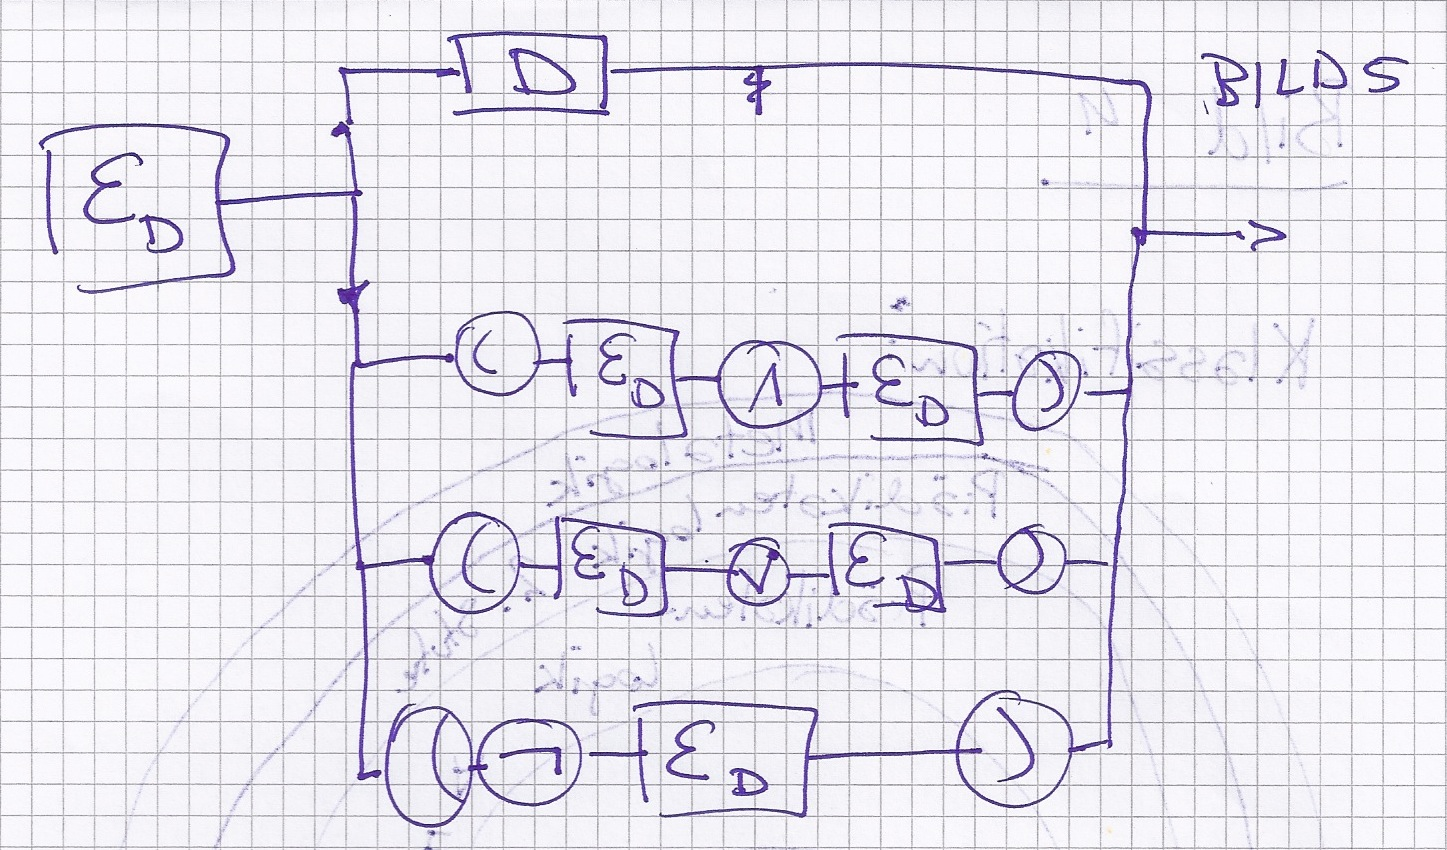
\includegraphics[width=\textwidth]{Bild7} \\
	Syntaktisch korrekte Formeln $\epsilon_D$ ist definiert über Atomformeln $D$:
	\begin{itemize}
		\item Atomformeln
		\item Falls $f$ und $g$ syntaktisch korrekt, dann auch $( \neg f ) , ( f \wedge g ) , ( f \vee g )$
		\item Das ist alles.
	\end{itemize}
\end{def*}
\begin{bsp*}
	\begin{itemize}
		\item $A$
		\item $( \neg A )$
		\item $( \neg ( \neg A ) )$
		\item $B$
		\item $( A \wedge B )$
		\item $( A \wedge A )$
		\item $( ( ( A \wedge B ) \vee ( \neg C ) ) \wedge ( A \vee B ) )$
	\end{itemize}
\end{bsp*}
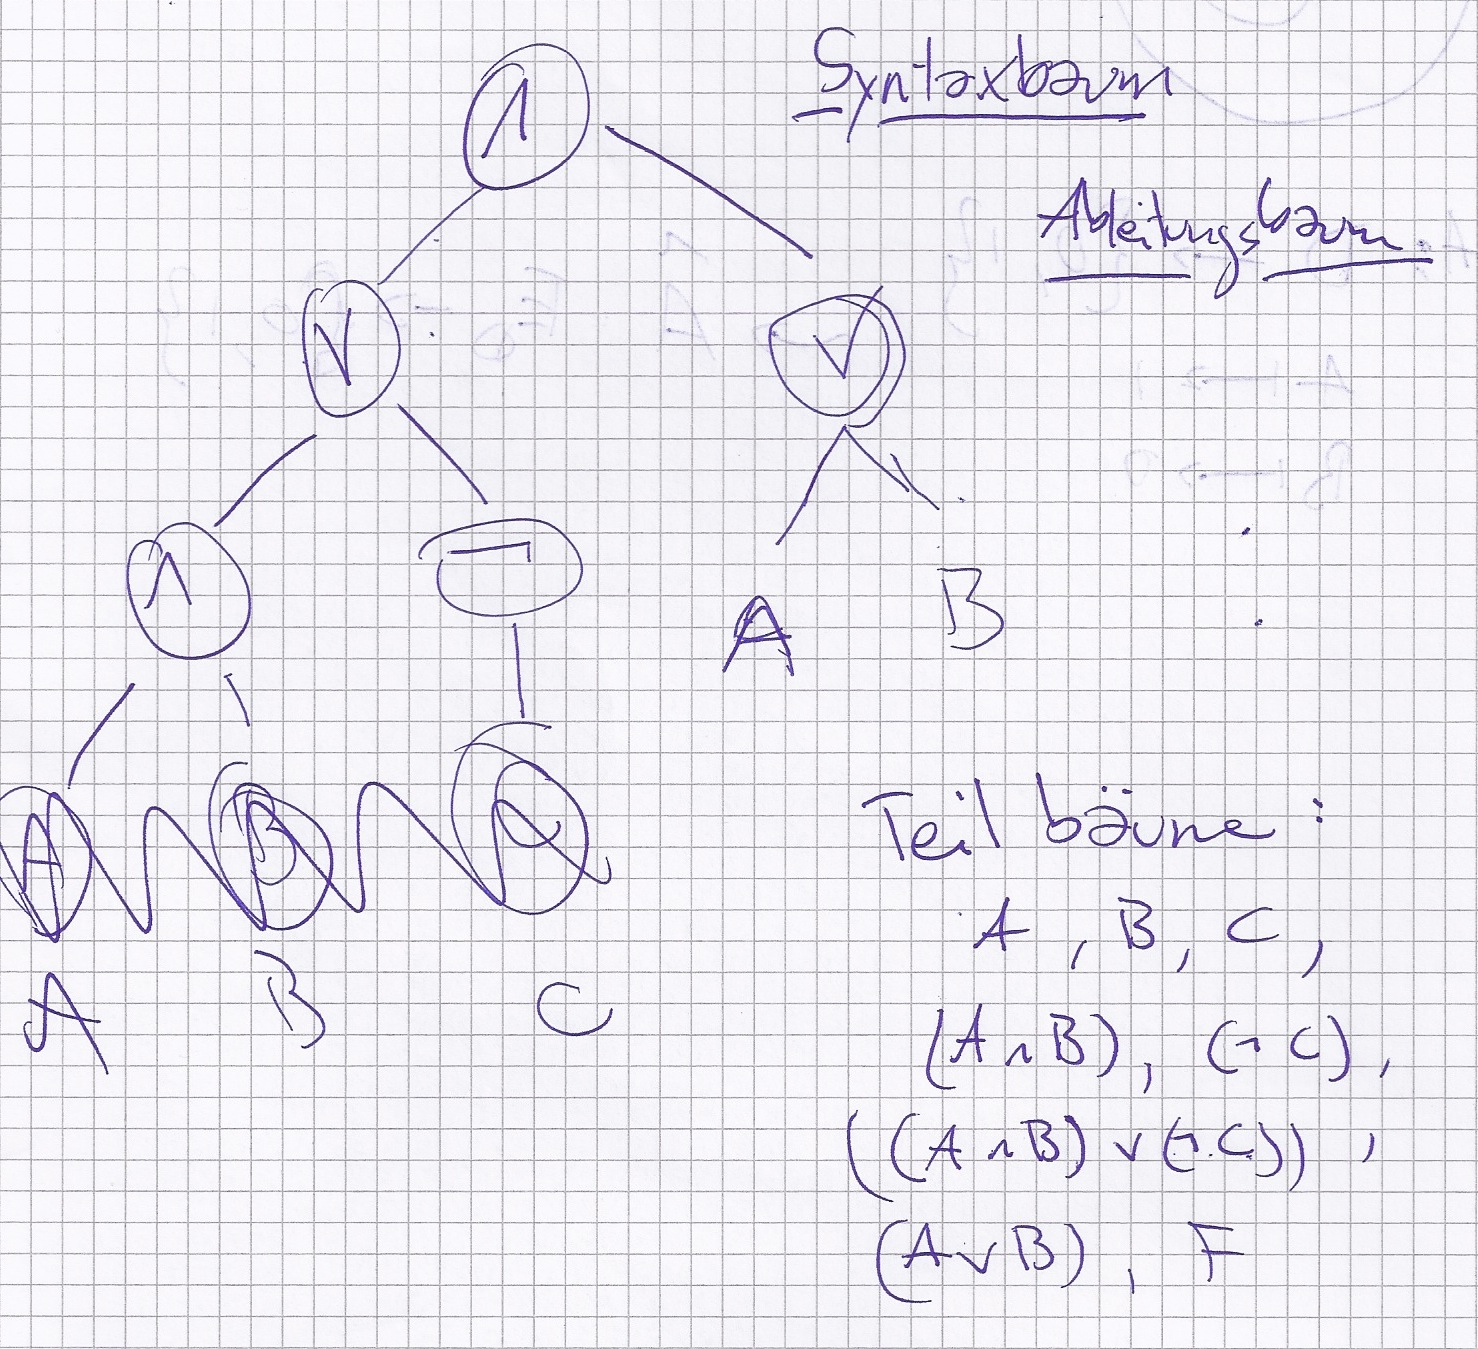
\includegraphics[width=\textwidth]{Bild8} \\
Teilformel = Teilstring, der selbst eine Formel ist. \\
\begin{bsp*}
	\begin{itemize}
		\item $A$
		\item $B$
		\item $C$
		\item $( A \wedge B )$
		\item $( \neg C )$
		\item $( ( A \wedge B ) \vee ( \neg C ) )$
		\item $( A \vee B )$
		\item $F$
	\end{itemize}
\end{bsp*}
